\documentclass[12pt,a4paper]{article}

\usepackage[left=3.00cm, right=2.00cm, top=2.00cm, bottom=2.00cm]{geometry}
\usepackage{lmodern}
\usepackage[T1]{fontenc}
\usepackage[utf8]{inputenc}
\usepackage[brazil]{babel}
\usepackage{microtype}

\usepackage{indentfirst,setspace}
\setlength{\parindent}{1.3cm}
\setlength{\parskip}{0.2cm}
\singlespacing

\usepackage{amssymb,amsmath,amsfonts}

\usepackage[numbers]{natbib}
\usepackage{url}
\bibliographystyle{plainnat}

\usepackage{longtable}
\usepackage{booktabs}
\usepackage[skip=1pt,labelfont=bf]{caption}
\usepackage{float}

\usepackage{listings}
\lstset{basicstyle=\ttfamily,frame=single}

\usepackage{graphicx}
\graphicspath{ {./imgs/} }

\numberwithin{figure}{section}
\numberwithin{table}{section}

\usepackage{lipsum}

\author{Pablo Cecilio Oliveira\\
Marcilene Reis}
\title{Primeiro Trabalho Prático de AOC I\\
Assembly MIPS}
\date{}

\begin{document}
\maketitle

\section{Introdução}

Mambojambo introduzindo sobre o que é o documento, as questões, Mars, etc.

\lipsum[1]

\section{Implementação}

\subsection{Questão 1}

O procedimento para calcular o $cosseno$ de um ângulo segundo a série de Taylor abaixo:
\[ \cos x = \sum_{n=0}^{\infty} \frac{(-1)^n}{(2n)!} x^{2n} \]

A função $seno$ chama funções para calcular o fatorial e a função potência de $x$. O usuário digita o ângulo em radianos e a quantidade de termos da série ($n>0$).

\subsection{Questão 2}

O programa lê uma \texttt{string} de um arquivo denominado \texttt{entrada.txt} e gera um novo arquivo de nome \texttt{saida.txt} contendo uma nova \texttt{string} processada. 

A \texttt{string} gerada no arquivo de saída possui seus caracteres maiúsculos trocados por minúsculos, e seus  caracteres minúsculos trocados por maiúsculos.

Para iniciar o processamento, inicialmente os dados dos arquivos a serem carregados são declarados, assim como é definido o espaço reservado para o buffer de leitura do arquivo de entrada.

\vspace{-0.5cm}
\begin{lstlisting}[caption={.data}]
.data
fin:     .asciiz "entrada.txt"
fout:    .asciiz "saida.txt"
string:  .space 1024
\end{lstlisting}

Inicia .text. A chamada para os procedimentos e a passagem das referencias.

\vspace{-0.5cm}
\begin{lstlisting}[caption={main}]
main:
la  $a0, fin
jal leArquivo
la  $a0, string
jal manipulaString
la  $a0, fout
jal salvaArquivo
li $v0, 10          # system call: Saia do programa
syscall             # Saia!
\end{lstlisting}

Procedimento \texttt{leArquivo} mais comentários a respeito de seu funcionamento por etapas e breve sumario de conclusão desse.

\vspace{-0.5cm}
\begin{lstlisting}[caption={leArquivo}]
leArquivo:
li   $v0, 13        # system call: Abre o arquivo
li   $a1, 0         # flag para somente leitura
li   $a2, 0         # modo ignorado
syscall             # Abra o arquivo!
move $t0, $v0       # Salva o descriptor em $t0
li   $v0, 14        # system call: Lendo o arquivo
move $a0, $t0       # Carrega o descriptor do arquivo
la   $a1, string    # endereco buffer
li   $a2, 255       # hardcoded buffer length
syscall             # Leia o arquivo!
move $s0, $v0       # Salva strlen em $s0
li   $v0, 16        # system call: Fecha o arquivo
syscall             # Feche o arquivo!
jr $ra
\end{lstlisting}


Procedimento \texttt{manipulaString} mais comentários a respeito de seu funcionamento por etapas e breve sumario de conclusão desse.

\lipsum[1]

\begin{table}[H]
	\renewcommand{\arraystretch}{1}
	\centering
	\caption{Tabela ASCII para A-Z e a-z}
	\label{tab:ascii}
	\begin{tabular}{rl|rl|rl|rl|rl|rl|rl}
		\toprule
		 65 & A &  69 & E &  73 & I &  77 & M &  81 & Q &  85 & U &  89 & Y \\
		 66 & B &  70 & F &  74 & J &  78 & N &  82 & R &  86 & V &  90 & Z \\
		 67 & C &  71 & G &  75 & K &  79 & O &  83 & S &  87 & W &     &   \\
		 68 & D &  72 & H &  76 & L &  80 & P &  84 & T &  88 & X &     &   \\
		\midrule
		 97 & a & 101 & e & 105 & i & 109 & m & 113 & q & 117 & u & 121 & y \\
		 98 & b & 102 & f & 106 & j & 110 & n & 114 & r & 118 & v & 122 & z \\
		 99 & c & 103 & g & 107 & k & 111 & o & 115 & s & 119 & w &     &   \\
		100 & d & 104 & h & 108 & l & 112 & p & 116 & t & 120 & x &     &   \\
		\bottomrule
		\multicolumn{12}{l}{\footnotesize Fonte: \citet*{wiki:xxx}}
	\end{tabular}
\end{table}

\vspace{-0.5cm}
\begin{lstlisting}[caption={manipulaString}]
manipulaString:
Loop:  
lb   $t2, ($a0)         # get the first byte pointed
beq  $t2, $zero, End    # if is equal to zero, End
slti $t1, $t2, 90       # if 'A-Z'
bne  $t1, $zero, Upper
slti $t1, $t2, 122      # if 'a-z'
bne  $t1, $zero, Lower
j Continue
Upper:
slti $t1, $t2, 65
bne  $t1, $zero, Continue
addi $t2, $t2, 32  
sb   $t2, ($a0)         # store it in the string
j Continue
Lower:
slti $t1, $t2, 97
bne  $t1, $zero, Continue
addi $t2, $t2, -32  
sb   $t2, ($a0)         # store it in the string
j Continue
Continue:               # Continue the iteration
addi $a0, $a0, 1        # Increment the address
j Loop
End:    
jr $ra
\end{lstlisting}

Procedimento \texttt{salvaArquivo} mais comentários a respeito de seu funcionamento por etapas e breve sumario de conclusão desse.

\pagebreak

\vspace{-0.5cm}
\begin{lstlisting}[caption={salvaArquivo}]
salvaArquivo:
li   $v0, 13        # system call: Abre o arquivo
li   $a1, 1         # flag para escrita
li   $a2, 0         # modo ignorado
syscall             # Abra o arquivo!
move $t0, $v0       # Salva o descriptor em $t0 
li   $v0, 15        # system call: Escrevendo no arquivo
move $a0, $t0       # Carrega o descriptor do arquivo 
la   $a1, string    # endereco do buffer
move $a2, $s0       # carrega strlen de $s0
syscall             # Escreva no arquivo!
li   $v0, 16        # system call: Fecha o arquivo
syscall             # Feche o arquivo!
jr $ra
\end{lstlisting}

\lipsum[1]

\begin{figure}[H]
	\centering
	\caption{Questão 2, estatísticas das instruções.}
	\vspace{0.2cm}
	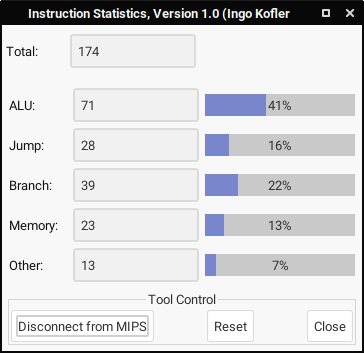
\includegraphics[width=242px]{questao2_stats}
	\\\footnotesize Fonte: Mars Instruction Statistic Tool
\end{figure}


\pagebreak

\begin{flushleft}
	\nocite{*}
	\bibliography{TP1}
	\vfill
	O histórico do desenvolvimento desse trabalho se encontra online em:\\ \url{https://github.com/Durfan/ufsj-aoc1-tp1}.
\end{flushleft}

\end{document}
